\documentclass[tikz,border=10pt]{standalone}
\begin{document}
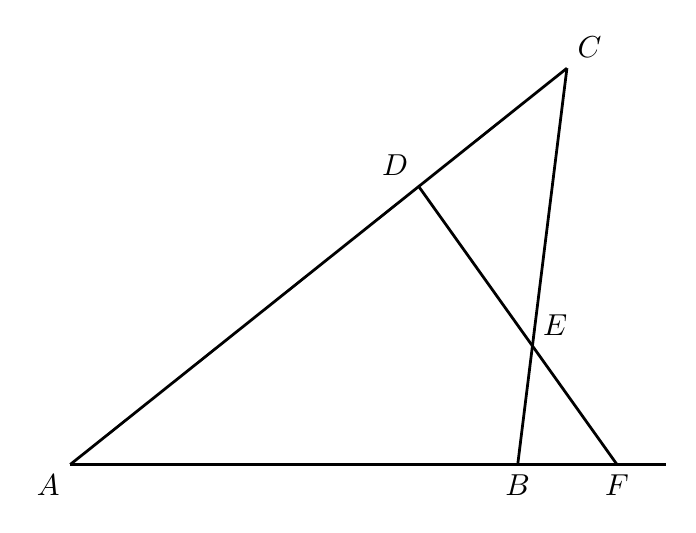
\begin{tikzpicture}[line join=round, line width=1.0pt,
  every node/.style={font=\fontsize{11}{13.2}\selectfont}]
\coordinate (A) at (-3.519,-2.379);
\coordinate (B) at (2.164,-2.379);
\coordinate (C) at (2.789,2.654);
\coordinate (D) at (0.907,1.152);
\coordinate (E) at (2.351,-0.873);
\coordinate (F) at (3.425,-2.379);




\draw (A) -- (D) -- (C);
\draw (A) -- (B) -- (F) -- (4.052,-2.379); 
\draw (B) -- (C);
\draw (D) -- (F);


\node[below left] at (A) {$A$};
\node[below] at (B) {$B$};
\node[below] at (F) {$F$};
\node[above right] at (C) {$C$};
\node[above left] at (D) {$D$};
\node[above right] at (E) {$E$};
\end{tikzpicture}
\end{document}